Also wird hier ausgetestet was passiert, wenn nicht kaskadiert wird. Da dies nur dann gut geht, wenn TF nicht verwendet wird, wird alles direkt 
auf dem Targetdatensatz gelernt. Die Netze werden so verändert, dass sie insgesamt gleich viele Hiddenlayer wie alle kleinen Netze, die im 
Direct Cascade Verfahren vorkommen, zusammen haben. Es werden dabei auch gleich viele Epochen insgesamt benutzt wie eben gerade. 

\begin{figure}[htpb]
    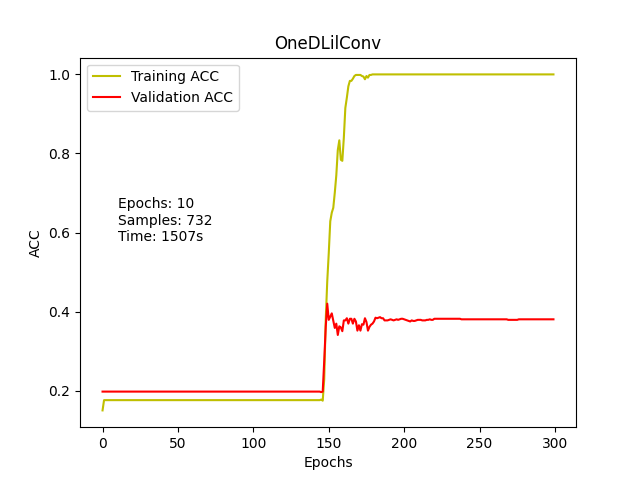
\includegraphics[height=5cm]{../../Plots/ba_plots/classnocascade/1dc.png}
    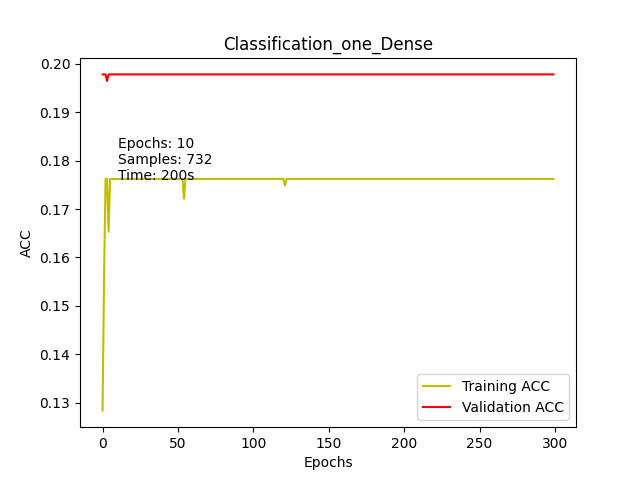
\includegraphics[height=5cm]{../../Plots/ba_plots/classnocascade/cod.png}
    \caption{\label{fig:nocascade} 
    \small{Hier sind Tests ohne Kaskadierung. Im genauen links: 1DC:Comp/732//30 und rechts: COD:Comp/732//30. Es ist zu sehen, wie der eine Plot 
    in ein lokales Maximum geraten ist und welcher maximale Accuracywert mit so wenigen Daten erwartbar wäre. Dieser wird nur mit den kompletten 
    hier aufgeführten Netzwerken erreicht.}}
\end{figure}

Was in der Figure 4.6 auffällt ist, dass es bei den meisten Epochen zu keinem Lerneffekt kommt. Ebenso kommt Overfitting vor, was bei so wenigen 
Daten zu erwarten ist. Obwohl hier nicht TF angewendet wird, gibt es in der Mitte des einen Plot einen plötzlichen Anstieg der Accuracy. 
Der Start dieser Verbesserung kam davon, dass der Validationwert minimal schlechter wurde, während der Trainingswert minimal besser wurde. 
Beide Veränderungen waren im Bereich von Zehnteln der Prozente. 
Deswegen scheint es so, dass es zu einem lokalen Maximum während des Trainings gekommen ist. Bei dem anderen Netz blieb der Wert auf dem des 
lokalen Maximums stehen, denn es sind die exakt gleichen Werte. Trotzdem wird durch Figure 4.6 klar, dass bei so wenigen Daten eine maximale 
Accuracy von 40\% zu erwarten ist. Dies ist das globale Maximum, da es den maximal möglichen Wert auf den Trainingsdaten vorweist. 
An diese kommt weder die Version des nur Kaskadierens noch die des Kaskadierens mit TF auch nur 
ansatzweise heran. Diese haben einen maximalen Wert von 20\% und sind somit nur halb so gut. 

Daraus folgt, dass es bereits an der Kaskadierung liegt, dass Klassifikation sinnlos mit TF in dem Direct Cascade Verfahren ist. 
Das kann dabei daran liegen, dass der CategoricalCrossEntropy sich selbst behindert, wenn dieser mehrfach genutzt wird. Sowie es auch an der 
Softmax-Aktivierungsfunktion oder die Art und Weise des Kaskadierens liegen könnte. 
